% Options for packages loaded elsewhere
\PassOptionsToPackage{unicode}{hyperref}
\PassOptionsToPackage{hyphens}{url}
%
\documentclass[
]{article}
\usepackage{amsmath,amssymb}
\usepackage{lmodern}
\usepackage{iftex}
\ifPDFTeX
  \usepackage[T1]{fontenc}
  \usepackage[utf8]{inputenc}
  \usepackage{textcomp} % provide euro and other symbols
\else % if luatex or xetex
  \usepackage{unicode-math}
  \defaultfontfeatures{Scale=MatchLowercase}
  \defaultfontfeatures[\rmfamily]{Ligatures=TeX,Scale=1}
\fi
% Use upquote if available, for straight quotes in verbatim environments
\IfFileExists{upquote.sty}{\usepackage{upquote}}{}
\IfFileExists{microtype.sty}{% use microtype if available
  \usepackage[]{microtype}
  \UseMicrotypeSet[protrusion]{basicmath} % disable protrusion for tt fonts
}{}
\makeatletter
\@ifundefined{KOMAClassName}{% if non-KOMA class
  \IfFileExists{parskip.sty}{%
    \usepackage{parskip}
  }{% else
    \setlength{\parindent}{0pt}
    \setlength{\parskip}{6pt plus 2pt minus 1pt}}
}{% if KOMA class
  \KOMAoptions{parskip=half}}
\makeatother
\usepackage{xcolor}
\usepackage[margin=1in]{geometry}
\usepackage{color}
\usepackage{fancyvrb}
\newcommand{\VerbBar}{|}
\newcommand{\VERB}{\Verb[commandchars=\\\{\}]}
\DefineVerbatimEnvironment{Highlighting}{Verbatim}{commandchars=\\\{\}}
% Add ',fontsize=\small' for more characters per line
\usepackage{framed}
\definecolor{shadecolor}{RGB}{248,248,248}
\newenvironment{Shaded}{\begin{snugshade}}{\end{snugshade}}
\newcommand{\AlertTok}[1]{\textcolor[rgb]{0.94,0.16,0.16}{#1}}
\newcommand{\AnnotationTok}[1]{\textcolor[rgb]{0.56,0.35,0.01}{\textbf{\textit{#1}}}}
\newcommand{\AttributeTok}[1]{\textcolor[rgb]{0.77,0.63,0.00}{#1}}
\newcommand{\BaseNTok}[1]{\textcolor[rgb]{0.00,0.00,0.81}{#1}}
\newcommand{\BuiltInTok}[1]{#1}
\newcommand{\CharTok}[1]{\textcolor[rgb]{0.31,0.60,0.02}{#1}}
\newcommand{\CommentTok}[1]{\textcolor[rgb]{0.56,0.35,0.01}{\textit{#1}}}
\newcommand{\CommentVarTok}[1]{\textcolor[rgb]{0.56,0.35,0.01}{\textbf{\textit{#1}}}}
\newcommand{\ConstantTok}[1]{\textcolor[rgb]{0.00,0.00,0.00}{#1}}
\newcommand{\ControlFlowTok}[1]{\textcolor[rgb]{0.13,0.29,0.53}{\textbf{#1}}}
\newcommand{\DataTypeTok}[1]{\textcolor[rgb]{0.13,0.29,0.53}{#1}}
\newcommand{\DecValTok}[1]{\textcolor[rgb]{0.00,0.00,0.81}{#1}}
\newcommand{\DocumentationTok}[1]{\textcolor[rgb]{0.56,0.35,0.01}{\textbf{\textit{#1}}}}
\newcommand{\ErrorTok}[1]{\textcolor[rgb]{0.64,0.00,0.00}{\textbf{#1}}}
\newcommand{\ExtensionTok}[1]{#1}
\newcommand{\FloatTok}[1]{\textcolor[rgb]{0.00,0.00,0.81}{#1}}
\newcommand{\FunctionTok}[1]{\textcolor[rgb]{0.00,0.00,0.00}{#1}}
\newcommand{\ImportTok}[1]{#1}
\newcommand{\InformationTok}[1]{\textcolor[rgb]{0.56,0.35,0.01}{\textbf{\textit{#1}}}}
\newcommand{\KeywordTok}[1]{\textcolor[rgb]{0.13,0.29,0.53}{\textbf{#1}}}
\newcommand{\NormalTok}[1]{#1}
\newcommand{\OperatorTok}[1]{\textcolor[rgb]{0.81,0.36,0.00}{\textbf{#1}}}
\newcommand{\OtherTok}[1]{\textcolor[rgb]{0.56,0.35,0.01}{#1}}
\newcommand{\PreprocessorTok}[1]{\textcolor[rgb]{0.56,0.35,0.01}{\textit{#1}}}
\newcommand{\RegionMarkerTok}[1]{#1}
\newcommand{\SpecialCharTok}[1]{\textcolor[rgb]{0.00,0.00,0.00}{#1}}
\newcommand{\SpecialStringTok}[1]{\textcolor[rgb]{0.31,0.60,0.02}{#1}}
\newcommand{\StringTok}[1]{\textcolor[rgb]{0.31,0.60,0.02}{#1}}
\newcommand{\VariableTok}[1]{\textcolor[rgb]{0.00,0.00,0.00}{#1}}
\newcommand{\VerbatimStringTok}[1]{\textcolor[rgb]{0.31,0.60,0.02}{#1}}
\newcommand{\WarningTok}[1]{\textcolor[rgb]{0.56,0.35,0.01}{\textbf{\textit{#1}}}}
\usepackage{graphicx}
\makeatletter
\def\maxwidth{\ifdim\Gin@nat@width>\linewidth\linewidth\else\Gin@nat@width\fi}
\def\maxheight{\ifdim\Gin@nat@height>\textheight\textheight\else\Gin@nat@height\fi}
\makeatother
% Scale images if necessary, so that they will not overflow the page
% margins by default, and it is still possible to overwrite the defaults
% using explicit options in \includegraphics[width, height, ...]{}
\setkeys{Gin}{width=\maxwidth,height=\maxheight,keepaspectratio}
% Set default figure placement to htbp
\makeatletter
\def\fps@figure{htbp}
\makeatother
\setlength{\emergencystretch}{3em} % prevent overfull lines
\providecommand{\tightlist}{%
  \setlength{\itemsep}{0pt}\setlength{\parskip}{0pt}}
\setcounter{secnumdepth}{5}
\ifLuaTeX
  \usepackage{selnolig}  % disable illegal ligatures
\fi
\IfFileExists{bookmark.sty}{\usepackage{bookmark}}{\usepackage{hyperref}}
\IfFileExists{xurl.sty}{\usepackage{xurl}}{} % add URL line breaks if available
\urlstyle{same} % disable monospaced font for URLs
\hypersetup{
  pdftitle={HUDM6122 Homework\_03},
  pdfauthor={Chenguang Pan},
  hidelinks,
  pdfcreator={LaTeX via pandoc}}

\title{HUDM6122 Homework\_03}
\author{Chenguang Pan}
\date{2023-02-19}

\begin{document}
\maketitle

\hypertarget{ex-3.1}{%
\subsection{Ex 3.1}\label{ex-3.1}}

\emph{Construct the scatterplot of the heptathlon data showing the
contours of the estimated bivariate density function on each panel. Is
this graphic more useful than the unenhanced scatterplot matrix?}

\textbf{MY SOLUTION:}

Here, I use the \texttt{MASS::kde2d()} function to estimate the
bivariate density of the data, and plot the contours of the density
using the \texttt{contour()} function.

\begin{Shaded}
\begin{Highlighting}[]
\SpecialCharTok{\textgreater{}} \CommentTok{\# import the package}
\ErrorTok{\textgreater{}} \FunctionTok{library}\NormalTok{(MVA)}
\SpecialCharTok{\textgreater{}} \FunctionTok{library}\NormalTok{(HSAUR2)}
\SpecialCharTok{\textgreater{}} \FunctionTok{data}\NormalTok{(heptathlon)}
\SpecialCharTok{\textgreater{}} \CommentTok{\# Create a scatterplot matrix with density contours}
\ErrorTok{\textgreater{}} \FunctionTok{pairs}\NormalTok{(heptathlon[, }\SpecialCharTok{{-}}\FunctionTok{ncol}\NormalTok{(heptathlon)], }\AttributeTok{upper.panel =} \ControlFlowTok{function}\NormalTok{(x, y) \{}
\SpecialCharTok{+}   \FunctionTok{points}\NormalTok{(x, y)}
\SpecialCharTok{+}\NormalTok{   den }\OtherTok{\textless{}{-}}\NormalTok{ MASS}\SpecialCharTok{::}\FunctionTok{kde2d}\NormalTok{(x, y)}
\SpecialCharTok{+}   \FunctionTok{contour}\NormalTok{(den, }\AttributeTok{add =} \ConstantTok{TRUE}\NormalTok{, }\AttributeTok{col =} \StringTok{"red"}\NormalTok{, }\AttributeTok{lwd =} \DecValTok{2}\NormalTok{)\})}
\end{Highlighting}
\end{Shaded}

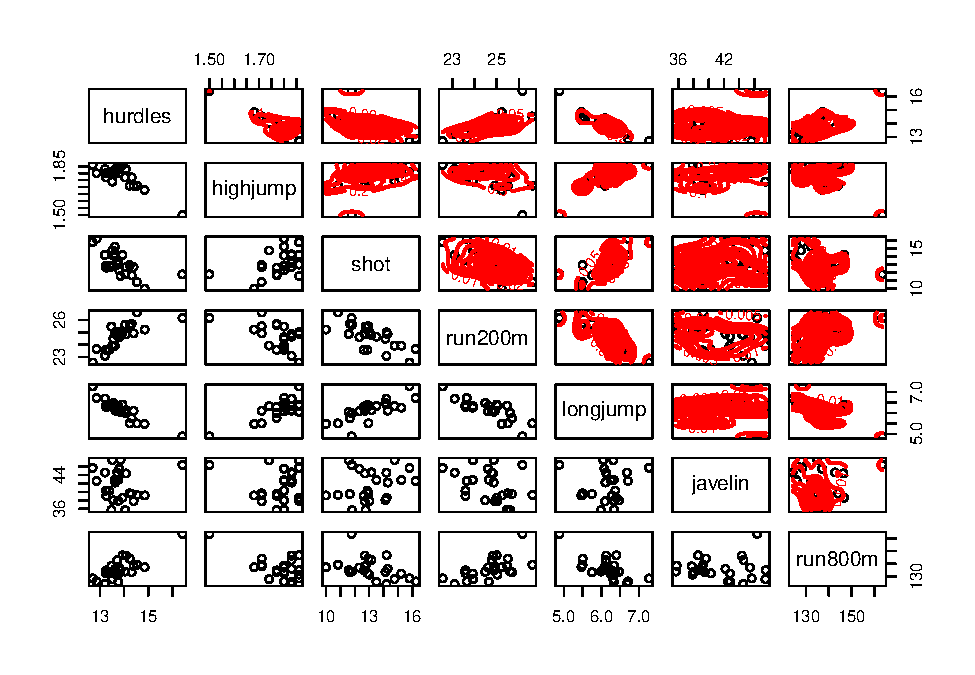
\includegraphics{HUDM6122-Homework_03-Chenguang-Pan_files/figure-latex/unnamed-chunk-1-1.pdf}

Comparing to the unenhanced scatter plot matrix, this mixed graph can
help to easily find the specific characteristics of joint distribution
of each pair, like the where is the center of the distribution.

\hypertarget{ex-3.2}{%
\subsection{Ex 3.2}\label{ex-3.2}}

\emph{Construct a diagram that shows the SO2 variable in the air
pollution data plotted against each of the six explanatory variables,
and in each of the scatterplots show the fitted linear regression and a
fitted locally weighted regression. Does this diagram help in deciding
on the most appropriate model for determining the variables most
predictive of sulphur dioxide levels?}

\textbf{MY SOLUTION:}

To solve this questions, I used the \texttt{ggplot2} to draw each graph.

\begin{Shaded}
\begin{Highlighting}[]
\SpecialCharTok{\textgreater{}} \CommentTok{\# try to use a for{-}loop to get all the maps in fewer lines}
\ErrorTok{\textgreater{}} \FunctionTok{par}\NormalTok{(}\AttributeTok{mfrow=}\FunctionTok{c}\NormalTok{(}\DecValTok{2}\NormalTok{,}\DecValTok{3}\NormalTok{))}
\SpecialCharTok{\textgreater{}} \ControlFlowTok{for}\NormalTok{ (i }\ControlFlowTok{in} \FunctionTok{c}\NormalTok{(}\DecValTok{2}\SpecialCharTok{:}\DecValTok{7}\NormalTok{)) \{}
\SpecialCharTok{+}\NormalTok{   p }\OtherTok{\textless{}{-}} \FunctionTok{ggplot}\NormalTok{(USairpollution, }\FunctionTok{aes}\NormalTok{(}\AttributeTok{x =}\NormalTok{ USairpollution[,i], }\AttributeTok{y =}\NormalTok{ SO2)) }\SpecialCharTok{+} 
\SpecialCharTok{+}                 \FunctionTok{geom\_point}\NormalTok{() }\SpecialCharTok{+}
\SpecialCharTok{+}                 \FunctionTok{geom\_smooth}\NormalTok{(}\AttributeTok{method =} \StringTok{"lm"}\NormalTok{, }\AttributeTok{se =} \ConstantTok{FALSE}\NormalTok{, }\AttributeTok{color =} \StringTok{"blue"}\NormalTok{) }\SpecialCharTok{+}
\SpecialCharTok{+}                 \FunctionTok{geom\_smooth}\NormalTok{(}\AttributeTok{span =} \DecValTok{1}\NormalTok{, }\AttributeTok{se =} \ConstantTok{FALSE}\NormalTok{, }\AttributeTok{color =} \StringTok{"red"}\NormalTok{) }\SpecialCharTok{+}
\SpecialCharTok{+}                 \FunctionTok{labs}\NormalTok{(}\AttributeTok{title =} \FunctionTok{paste0}\NormalTok{(}\StringTok{"SO2 vs "}\NormalTok{, }\FunctionTok{colnames}\NormalTok{(USairpollution)[i]))}\SpecialCharTok{+}
\SpecialCharTok{+}                 \CommentTok{\# to remove the un{-}elegant x{-}axis name}
\SpecialCharTok{+}                 \FunctionTok{theme}\NormalTok{(}\AttributeTok{axis.title.x =} \FunctionTok{element\_blank}\NormalTok{(),}
\SpecialCharTok{+}                       \AttributeTok{axis.text.x =} \FunctionTok{element\_blank}\NormalTok{(),}
\SpecialCharTok{+}                       \AttributeTok{axis.ticks.x =} \FunctionTok{element\_blank}\NormalTok{())}
\SpecialCharTok{+}   \CommentTok{\# assign(var\_name, p)}
\SpecialCharTok{+}   \FunctionTok{print}\NormalTok{(p)}
\SpecialCharTok{+}\NormalTok{ \}}
\end{Highlighting}
\end{Shaded}

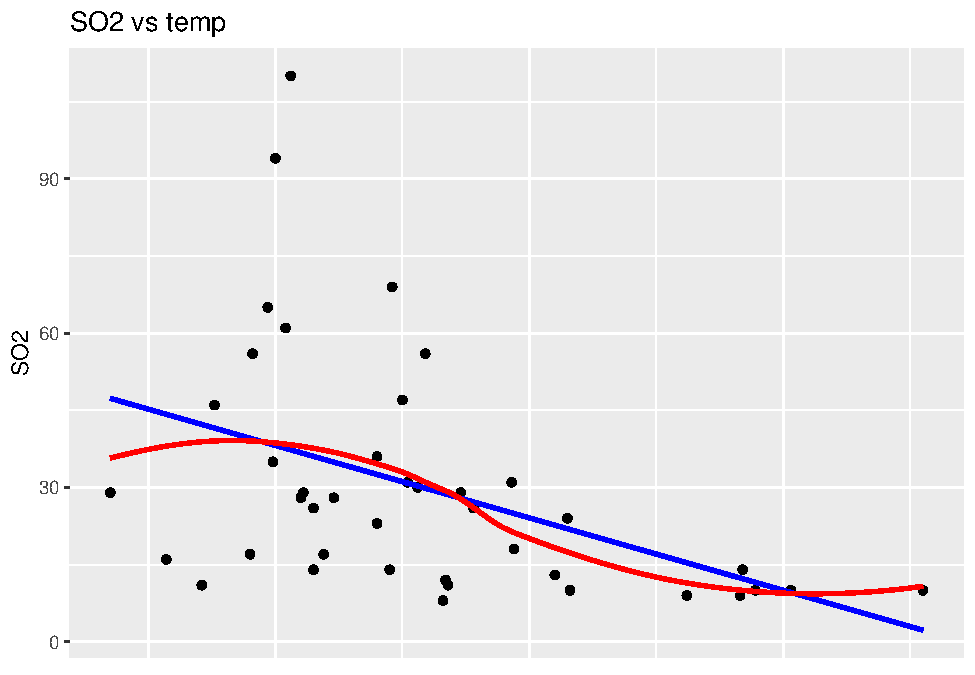
\includegraphics[width=0.5\linewidth,height=0.33\textheight]{HUDM6122-Homework_03-Chenguang-Pan_files/figure-latex/unnamed-chunk-3-1}
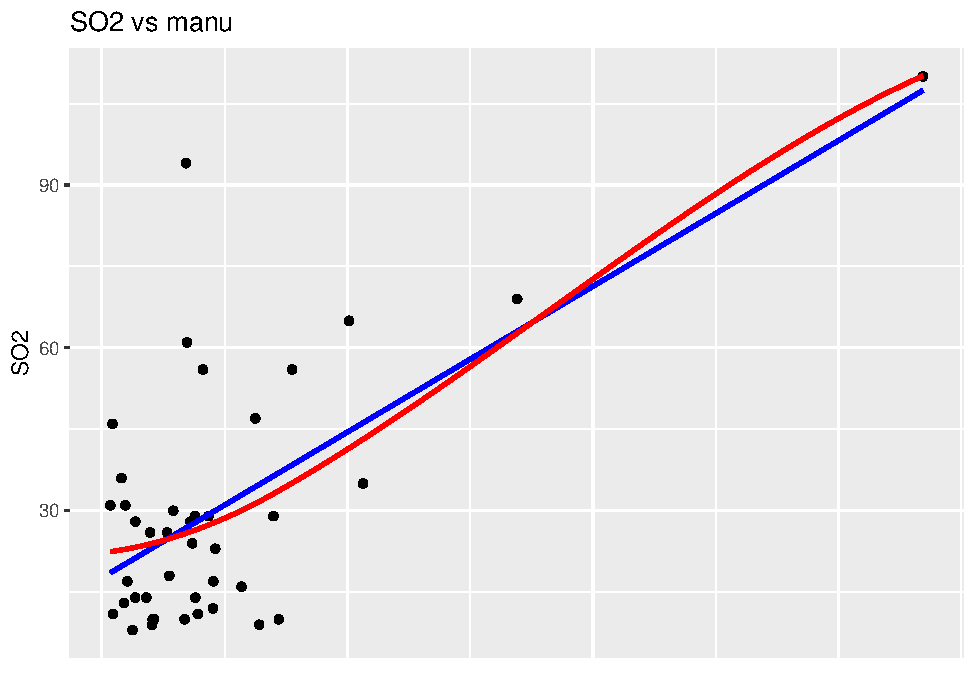
\includegraphics[width=0.5\linewidth,height=0.33\textheight]{HUDM6122-Homework_03-Chenguang-Pan_files/figure-latex/unnamed-chunk-3-2}
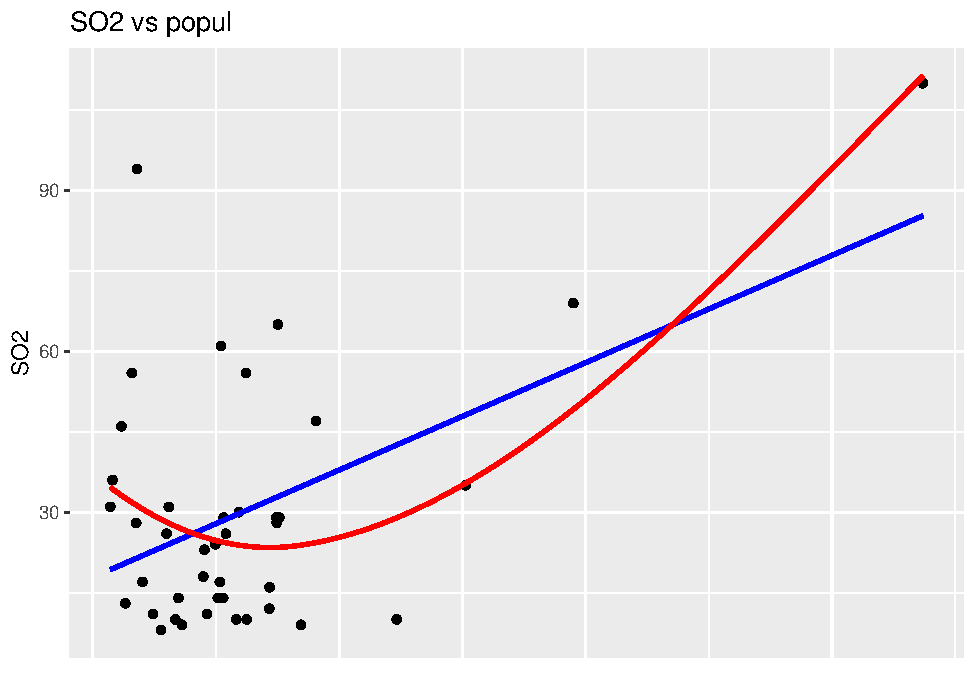
\includegraphics[width=0.5\linewidth,height=0.33\textheight]{HUDM6122-Homework_03-Chenguang-Pan_files/figure-latex/unnamed-chunk-3-3}
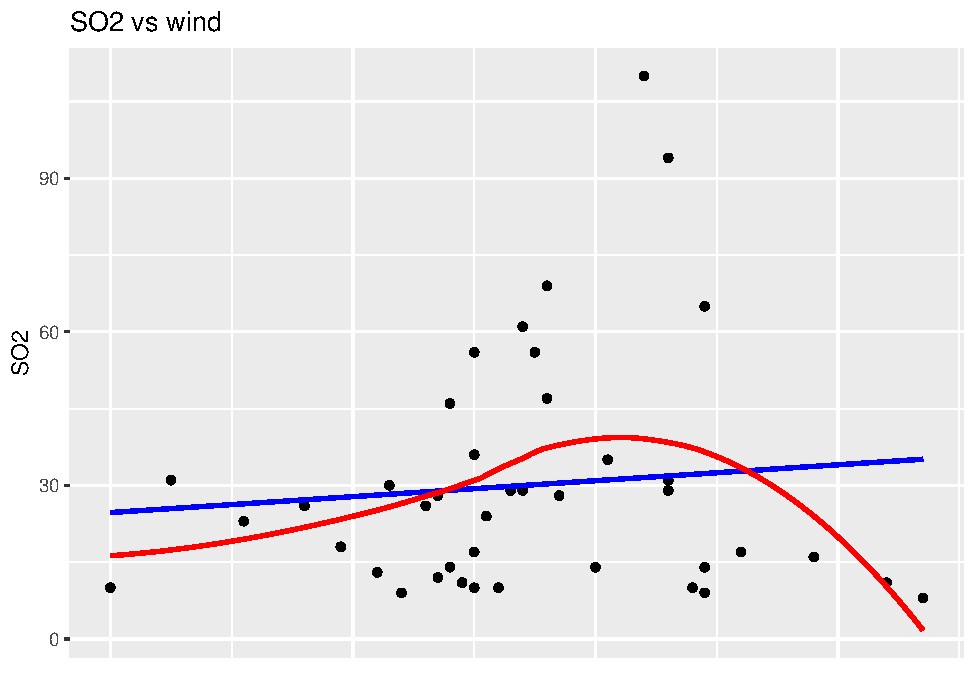
\includegraphics[width=0.5\linewidth,height=0.33\textheight]{HUDM6122-Homework_03-Chenguang-Pan_files/figure-latex/unnamed-chunk-3-4}
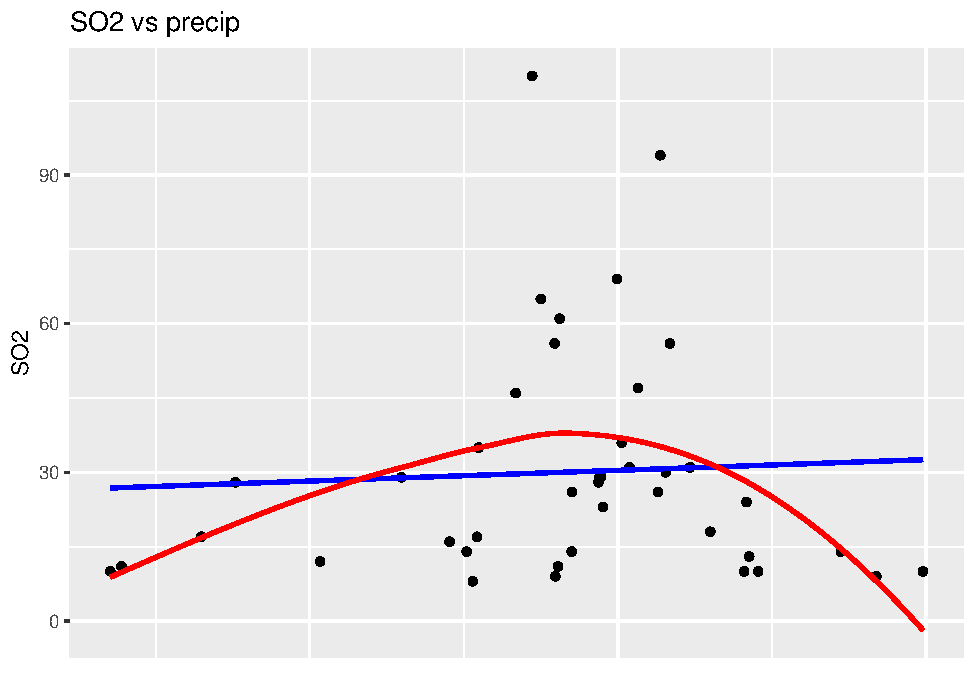
\includegraphics[width=0.5\linewidth,height=0.33\textheight]{HUDM6122-Homework_03-Chenguang-Pan_files/figure-latex/unnamed-chunk-3-5}
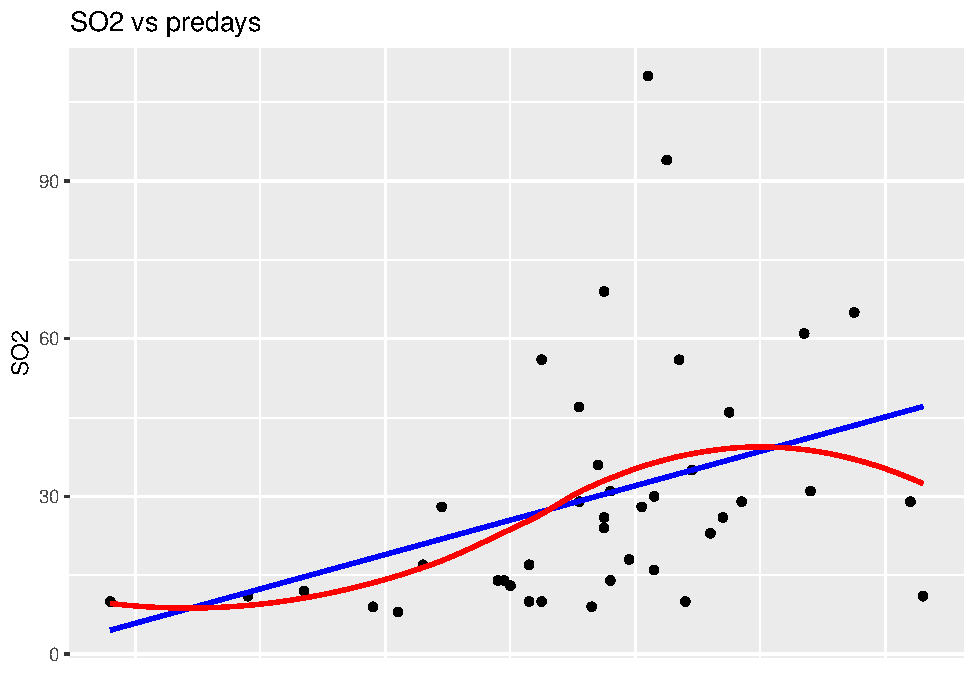
\includegraphics[width=0.5\linewidth,height=0.33\textheight]{HUDM6122-Homework_03-Chenguang-Pan_files/figure-latex/unnamed-chunk-3-6}
From six graphs above, we can not easily tell what the strongest
predictor is for predicting the \(SO_2\) concentration, since there are
some outliers with high leverage in each graph.

\hypertarget{ex-3.3}{%
\subsection{Ex 3.3}\label{ex-3.3}}

\emph{Find the principal components of the following correlation matrix
given by MacDonnell (1902) from measurements of seven physical char-
acteristics in each of 3000 convicted criminals: How would you interpret
the derived components?}

\textbf{MY SOLUTION}\\
First, by using \texttt{forceSymmetric()} function in the package
\texttt{Matrix} to transform the low triangular correlation matrix into
a complete correlation matrix. And then, I use \texttt{prcomp()} to get
the components.

\begin{Shaded}
\begin{Highlighting}[]
\SpecialCharTok{\textgreater{}} \FunctionTok{library}\NormalTok{(Matrix)}
\SpecialCharTok{\textgreater{}} \CommentTok{\# import the correlation matrix}
\ErrorTok{\textgreater{}}\NormalTok{ corr\_lower }\OtherTok{\textless{}{-}} \FunctionTok{matrix}\NormalTok{(}\FunctionTok{c}\NormalTok{(}\DecValTok{1}\NormalTok{, }\DecValTok{0}\NormalTok{, }\DecValTok{0}\NormalTok{, }\DecValTok{0}\NormalTok{, }\DecValTok{0}\NormalTok{, }\DecValTok{0}\NormalTok{, }\DecValTok{0}\NormalTok{,}
\SpecialCharTok{+}                       \FloatTok{0.402}\NormalTok{, }\DecValTok{1}\NormalTok{, }\DecValTok{0}\NormalTok{,}\DecValTok{0}\NormalTok{,}\DecValTok{0}\NormalTok{,}\DecValTok{0}\NormalTok{,}\DecValTok{0}\NormalTok{,}
\SpecialCharTok{+}                       \FloatTok{0.396}\NormalTok{, }\FloatTok{0.618}\NormalTok{, }\DecValTok{1}\NormalTok{,}\DecValTok{0}\NormalTok{,}\DecValTok{0}\NormalTok{,}\DecValTok{0}\NormalTok{,}\DecValTok{0}\NormalTok{,}
\SpecialCharTok{+}                       \FloatTok{0.301}\NormalTok{, }\FloatTok{0.150}\NormalTok{, }\FloatTok{0.321}\NormalTok{, }\DecValTok{1}\NormalTok{,}\DecValTok{0}\NormalTok{,}\DecValTok{0}\NormalTok{,}\DecValTok{0}\NormalTok{,}
\SpecialCharTok{+}                       \FloatTok{0.305}\NormalTok{, }\FloatTok{0.135}\NormalTok{, }\FloatTok{0.289}\NormalTok{, }\FloatTok{0.846}\NormalTok{, }\DecValTok{1}\NormalTok{,}\DecValTok{0}\NormalTok{,}\DecValTok{0}\NormalTok{,}
\SpecialCharTok{+}                       \FloatTok{0.339}\NormalTok{, }\FloatTok{0.206}\NormalTok{, }\FloatTok{0.363}\NormalTok{, }\FloatTok{0.759}\NormalTok{, }\FloatTok{0.797}\NormalTok{, }\DecValTok{1}\NormalTok{,}\DecValTok{0}\NormalTok{,}
\SpecialCharTok{+}                       \FloatTok{0.340}\NormalTok{, }\FloatTok{0.183}\NormalTok{, }\FloatTok{0.345}\NormalTok{, }\FloatTok{0.661}\NormalTok{, }\FloatTok{0.800}\NormalTok{, }\FloatTok{0.736}\NormalTok{, }\DecValTok{1}\NormalTok{),}\DecValTok{7}\NormalTok{,}\DecValTok{7}\NormalTok{, }\AttributeTok{byrow =}\NormalTok{ T)}
\SpecialCharTok{\textgreater{}} \CommentTok{\# generate a complete correlation matrix}
\ErrorTok{\textgreater{}}\NormalTok{ corr\_symmetric }\OtherTok{\textless{}{-}} \FunctionTok{forceSymmetric}\NormalTok{(corr\_lower, }\AttributeTok{uplo=}\StringTok{"L"}\NormalTok{)}
\SpecialCharTok{\textgreater{}} \CommentTok{\# use prcomp to calculate the principal components}
\ErrorTok{\textgreater{}}\NormalTok{ pca }\OtherTok{\textless{}{-}} \FunctionTok{prcomp}\NormalTok{(corr\_symmetric, }\AttributeTok{scale. =} \ConstantTok{FALSE}\NormalTok{)}
\SpecialCharTok{\textgreater{}} \CommentTok{\# get the PCA results}
\ErrorTok{\textgreater{}} \FunctionTok{summary}\NormalTok{(pca)}
\NormalTok{Importance of components}\SpecialCharTok{:}
\NormalTok{                          PC1    PC2     PC3     PC4     PC5     PC6       PC7}
\NormalTok{Standard deviation     }\FloatTok{0.7063} \FloatTok{0.2677} \FloatTok{0.15376} \FloatTok{0.13851} \FloatTok{0.09832} \FloatTok{0.04686} \FloatTok{3.458e{-}17}
\NormalTok{Proportion of Variance }\FloatTok{0.7979} \FloatTok{0.1146} \FloatTok{0.03781} \FloatTok{0.03069} \FloatTok{0.01546} \FloatTok{0.00351} \FloatTok{0.000e+00}
\NormalTok{Cumulative Proportion  }\FloatTok{0.7979} \FloatTok{0.9125} \FloatTok{0.95034} \FloatTok{0.98103} \FloatTok{0.99649} \FloatTok{1.00000} \FloatTok{1.000e+00}
\SpecialCharTok{\textgreater{}} \CommentTok{\# draw the scree plot }
\ErrorTok{\textgreater{}} \FunctionTok{plot}\NormalTok{(pca, }\AttributeTok{type =} \StringTok{"l"}\NormalTok{, }
\SpecialCharTok{+}      \AttributeTok{main =} \StringTok{"Scree Plot"}\NormalTok{)}
\end{Highlighting}
\end{Shaded}

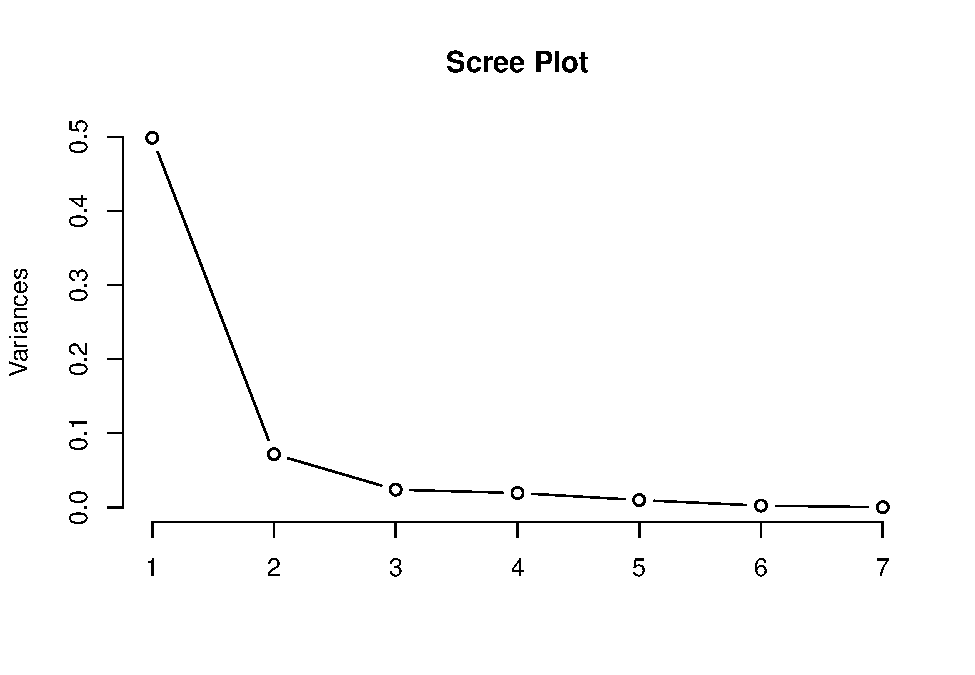
\includegraphics[width=0.7\linewidth,height=0.5\textheight]{HUDM6122-Homework_03-Chenguang-Pan_files/figure-latex/unnamed-chunk-4-1}

The first two components can explain 91.25\% variance of the total.
Therefore, I will choose to use the first two components to represent
this dataset.

\hypertarget{ex-3.4}{%
\subsection{Ex 3.4}\label{ex-3.4}}

\emph{Not all canonical correlations may be statistically significant.
An approximate test proposed by Bartlett (1947) can be used to deter-
mine how many significant relationships exist. The test statistic for
testing that at least one canonical correlation is significant is}

\textbf{MY SOLUTION}\\
This dataset is called \texttt{frets} included in the package
\texttt{boot}. The \texttt{l1} and \texttt{l2} variables represent the
length and the \texttt{b1} and \texttt{b2} are for the breadth. The
index number \texttt{1} represents the first son and \texttt{2} for the
second son in one family. Note, the code for \texttt{headsize.std}
provided on \emph{Page.97} in the textbook MVA is \textbf{wrong}! Each
columns divided by the standard deviation cannot be called
``standardized''! One should let each column subtract the mean first!!

First, I write a function to calculate the chi-square value. Although
the book does not mention, one should notice that the \texttt{n}is the
number of observations.

\begin{Shaded}
\begin{Highlighting}[]
\SpecialCharTok{\textgreater{}}\NormalTok{ cc\_test }\OtherTok{\textless{}{-}} \ControlFlowTok{function}\NormalTok{(eigenvalues, n, q1,q2)\{}
\SpecialCharTok{+}   \CommentTok{\# eigenvalues is a list of a eigenvalues computed by hand.}
\SpecialCharTok{+}   \CommentTok{\# s\_df is the df of the s matrix, ie., the n in the equation}
\SpecialCharTok{+}   \CommentTok{\# p\_q is}
\SpecialCharTok{+}   \CommentTok{\# write a for{-}loop to load the sum of log eigenvalues}
\SpecialCharTok{+}\NormalTok{   sum\_log\_eigen }\OtherTok{\textless{}{-}} \DecValTok{0}
\SpecialCharTok{+}   \ControlFlowTok{for}\NormalTok{ (i }\ControlFlowTok{in} \FunctionTok{c}\NormalTok{(}\DecValTok{1}\SpecialCharTok{:}\FunctionTok{min}\NormalTok{(q1,q2))) \{}
\SpecialCharTok{+}\NormalTok{     sum\_log\_eigen }\OtherTok{\textless{}{-}}\NormalTok{ sum\_log\_eigen }\SpecialCharTok{+} \FunctionTok{log}\NormalTok{(}\DecValTok{1}\SpecialCharTok{{-}}\NormalTok{eigenvalues[i])}
\SpecialCharTok{+}\NormalTok{   \}}
\SpecialCharTok{+} 
\SpecialCharTok{+}\NormalTok{   phi\_2 }\OtherTok{\textless{}{-}} \SpecialCharTok{{-}}\NormalTok{(n }\SpecialCharTok{{-}} \FloatTok{0.5}\SpecialCharTok{*}\NormalTok{(q1}\SpecialCharTok{+}\NormalTok{q2}\SpecialCharTok{+}\DecValTok{1}\NormalTok{))}\SpecialCharTok{*}\NormalTok{sum\_log\_eigen}
\SpecialCharTok{+}\NormalTok{   p\_value }\OtherTok{\textless{}{-}} \FunctionTok{pchisq}\NormalTok{(}\AttributeTok{q =}\NormalTok{ phi\_2, }\AttributeTok{df =}\NormalTok{ q1}\SpecialCharTok{*}\NormalTok{q2, }\AttributeTok{lower.tail =}\NormalTok{ F)}
\SpecialCharTok{+}   \FunctionTok{return}\NormalTok{(p\_value)}
\SpecialCharTok{+}\NormalTok{ \}}
\end{Highlighting}
\end{Shaded}

Write separate code chunk to calculate the eigenvalues of
\texttt{headsize} dataset. Based on the dimension of dataset, we can
easily find the \texttt{q1} = 2, \texttt{q2} = 2, and the df of s matrix
is

\begin{Shaded}
\begin{Highlighting}[]
\SpecialCharTok{\textgreater{}} \CommentTok{\# import the data}
\ErrorTok{\textgreater{}} \FunctionTok{data}\NormalTok{(}\StringTok{"frets"}\NormalTok{, }\AttributeTok{package =} \StringTok{"boot"}\NormalTok{)}
\SpecialCharTok{\textgreater{}}\NormalTok{ headsize }\OtherTok{\textless{}{-}}\NormalTok{ frets}
\SpecialCharTok{\textgreater{}} \CommentTok{\# use scale to get the standardized headsize dataset}
\ErrorTok{\textgreater{}}\NormalTok{ headsize\_std }\OtherTok{\textless{}{-}} \FunctionTok{as.data.frame}\NormalTok{(}\FunctionTok{scale}\NormalTok{(headsize))}
\SpecialCharTok{\textgreater{}} \CommentTok{\# get the correlation matrix}
\ErrorTok{\textgreater{}}\NormalTok{ R }\OtherTok{\textless{}{-}} \FunctionTok{cor}\NormalTok{(headsize\_std)}
\SpecialCharTok{\textgreater{}} \CommentTok{\# subset the correlation matrix to get the cor matrix for all first son}
\ErrorTok{\textgreater{}}\NormalTok{ r11 }\OtherTok{\textless{}{-}}\NormalTok{ R[}\DecValTok{1}\SpecialCharTok{:}\DecValTok{2}\NormalTok{, }\DecValTok{1}\SpecialCharTok{:}\DecValTok{2}\NormalTok{]}
\SpecialCharTok{\textgreater{}}\NormalTok{ r22 }\OtherTok{\textless{}{-}}\NormalTok{ R[}\SpecialCharTok{{-}}\NormalTok{(}\DecValTok{1}\SpecialCharTok{:}\DecValTok{2}\NormalTok{), }\SpecialCharTok{{-}}\NormalTok{(}\DecValTok{1}\SpecialCharTok{:}\DecValTok{2}\NormalTok{)]}
\SpecialCharTok{\textgreater{}}\NormalTok{ r12 }\OtherTok{\textless{}{-}}\NormalTok{ R[}\DecValTok{1}\SpecialCharTok{:}\DecValTok{2}\NormalTok{, }\SpecialCharTok{{-}}\NormalTok{(}\DecValTok{1}\SpecialCharTok{:}\DecValTok{2}\NormalTok{)]}
\SpecialCharTok{\textgreater{}}\NormalTok{ r21 }\OtherTok{\textless{}{-}}\NormalTok{ R[}\SpecialCharTok{{-}}\NormalTok{(}\DecValTok{1}\SpecialCharTok{:}\DecValTok{2}\NormalTok{), }\DecValTok{1}\SpecialCharTok{:}\DecValTok{2}\NormalTok{]}
\SpecialCharTok{\textgreater{}} \CommentTok{\# since the eigenvalues are the same for E1 and E2, here I only compute E1}
\ErrorTok{\textgreater{}}\NormalTok{ E1 }\OtherTok{\textless{}{-}} \FunctionTok{solve}\NormalTok{(r11)}\SpecialCharTok{\%*\%}\NormalTok{r12}\SpecialCharTok{\%*\%}\FunctionTok{solve}\NormalTok{(r22)}\SpecialCharTok{\%*\%}\NormalTok{r21}
\SpecialCharTok{\textgreater{}}\NormalTok{ E2 }\OtherTok{\textless{}{-}} \FunctionTok{solve}\NormalTok{(r22)}\SpecialCharTok{\%*\%}\NormalTok{r21}\SpecialCharTok{\%*\%}\FunctionTok{solve}\NormalTok{(r11)}\SpecialCharTok{\%*\%}\NormalTok{r12}
\SpecialCharTok{\textgreater{}} \CommentTok{\# get the eigenvector of two dataset}
\ErrorTok{\textgreater{}}\NormalTok{ e1 }\OtherTok{\textless{}{-}} \FunctionTok{eigen}\NormalTok{(E1)}\SpecialCharTok{$}\NormalTok{values}
\SpecialCharTok{\textgreater{}}\NormalTok{ e2 }\OtherTok{\textless{}{-}} \FunctionTok{eigen}\NormalTok{(E2)}\SpecialCharTok{$}\NormalTok{values}
\end{Highlighting}
\end{Shaded}

Now, plug the values from the analysis above to the initial
\texttt{cc\_test} function.

\begin{Shaded}
\begin{Highlighting}[]
\SpecialCharTok{\textgreater{}} \FunctionTok{cc\_test}\NormalTok{(e1, }\CommentTok{\# the eigenvalues are quite identical, here I use e1}
\SpecialCharTok{+}         \DecValTok{25}\NormalTok{, }\CommentTok{\# number of observations}
\SpecialCharTok{+}         \DecValTok{2}\NormalTok{, }\CommentTok{\# number of q1}
\SpecialCharTok{+}         \DecValTok{2}\NormalTok{) }\CommentTok{\# number of q2}
\NormalTok{[}\DecValTok{1}\NormalTok{] }\FloatTok{0.0002060779}
\end{Highlighting}
\end{Shaded}

The p value of a chi-square test at the degree of freedom 4 is far less
than than the significant level .05. Therefore, we reject the null
hypothesis. That is, at least one of the canonical correlation is
significant.

Follow the same method, I first analyzed the dataset \texttt{LAdepr} to
get the basic information and then plug them into the \texttt{cc\_test}.

\begin{Shaded}
\begin{Highlighting}[]
\SpecialCharTok{\textgreater{}} \CommentTok{\# import the data}
\ErrorTok{\textgreater{}}\NormalTok{ depr }\OtherTok{\textless{}{-}} \FunctionTok{c}\NormalTok{(}
\SpecialCharTok{+}            \FloatTok{0.212}\NormalTok{,}
\SpecialCharTok{+}            \FloatTok{0.124}\NormalTok{,  }\FloatTok{0.098}\NormalTok{,}
\SpecialCharTok{+}           \SpecialCharTok{{-}}\FloatTok{0.164}\NormalTok{,  }\FloatTok{0.308}\NormalTok{,  }\FloatTok{0.044}\NormalTok{,}
\SpecialCharTok{+}           \SpecialCharTok{{-}}\FloatTok{0.101}\NormalTok{, }\SpecialCharTok{{-}}\FloatTok{0.207}\NormalTok{, }\SpecialCharTok{{-}}\FloatTok{0.106}\NormalTok{, }\SpecialCharTok{{-}}\FloatTok{0.208}\NormalTok{,}
\SpecialCharTok{+}           \SpecialCharTok{{-}}\FloatTok{0.158}\NormalTok{, }\SpecialCharTok{{-}}\FloatTok{0.183}\NormalTok{, }\SpecialCharTok{{-}}\FloatTok{0.180}\NormalTok{, }\SpecialCharTok{{-}}\FloatTok{0.192}\NormalTok{, }\FloatTok{0.492}\NormalTok{)}
\SpecialCharTok{\textgreater{}}\NormalTok{ LAdepr }\OtherTok{\textless{}{-}} \FunctionTok{diag}\NormalTok{(}\DecValTok{6}\NormalTok{) }\SpecialCharTok{/} \DecValTok{2}
\SpecialCharTok{\textgreater{}}\NormalTok{ LAdepr[}\FunctionTok{upper.tri}\NormalTok{(LAdepr)] }\OtherTok{\textless{}{-}}\NormalTok{ depr}
\SpecialCharTok{\textgreater{}}\NormalTok{ LAdepr }\OtherTok{\textless{}{-}}\NormalTok{ LAdepr }\SpecialCharTok{+} \FunctionTok{t}\NormalTok{(LAdepr)}
\SpecialCharTok{\textgreater{}} \FunctionTok{rownames}\NormalTok{(LAdepr) }\OtherTok{\textless{}{-}} \FunctionTok{colnames}\NormalTok{(LAdepr) }\OtherTok{\textless{}{-}} \FunctionTok{c}\NormalTok{(}\StringTok{"CESD"}\NormalTok{, }\StringTok{"Health"}\NormalTok{, }\StringTok{"Gender"}\NormalTok{, }\StringTok{"Age"}\NormalTok{, }\StringTok{"Edu"}\NormalTok{, }\StringTok{"Income"}\NormalTok{)}
\SpecialCharTok{\textgreater{}} \CommentTok{\# LAdepr \textless{}{-} as.data.frame(LAdepr)}
\ErrorTok{\textgreater{}}\NormalTok{ r11 }\OtherTok{\textless{}{-}}\NormalTok{ LAdepr[}\DecValTok{1}\SpecialCharTok{:}\DecValTok{2}\NormalTok{, }\DecValTok{1}\SpecialCharTok{:}\DecValTok{2}\NormalTok{]}
\SpecialCharTok{\textgreater{}}\NormalTok{ r22 }\OtherTok{\textless{}{-}}\NormalTok{ LAdepr[}\SpecialCharTok{{-}}\NormalTok{(}\DecValTok{1}\SpecialCharTok{:}\DecValTok{2}\NormalTok{), }\SpecialCharTok{{-}}\NormalTok{(}\DecValTok{1}\SpecialCharTok{:}\DecValTok{2}\NormalTok{)]}
\SpecialCharTok{\textgreater{}}\NormalTok{ r12 }\OtherTok{\textless{}{-}}\NormalTok{ LAdepr[}\DecValTok{1}\SpecialCharTok{:}\DecValTok{2}\NormalTok{, }\SpecialCharTok{{-}}\NormalTok{(}\DecValTok{1}\SpecialCharTok{:}\DecValTok{2}\NormalTok{)]}
\SpecialCharTok{\textgreater{}}\NormalTok{ r21 }\OtherTok{\textless{}{-}}\NormalTok{ LAdepr[}\SpecialCharTok{{-}}\NormalTok{(}\DecValTok{1}\SpecialCharTok{:}\DecValTok{2}\NormalTok{), }\DecValTok{1}\SpecialCharTok{:}\DecValTok{2}\NormalTok{]}
\SpecialCharTok{\textgreater{}}\NormalTok{ E1 }\OtherTok{\textless{}{-}} \FunctionTok{solve}\NormalTok{(r11)}\SpecialCharTok{\%*\%}\NormalTok{r12}\SpecialCharTok{\%*\%}\FunctionTok{solve}\NormalTok{(r22)}\SpecialCharTok{\%*\%}\NormalTok{r21}
\SpecialCharTok{\textgreater{}}\NormalTok{ E2 }\OtherTok{\textless{}{-}} \FunctionTok{solve}\NormalTok{(r22)}\SpecialCharTok{\%*\%}\NormalTok{r21}\SpecialCharTok{\%*\%}\FunctionTok{solve}\NormalTok{(r11)}\SpecialCharTok{\%*\%}\NormalTok{r12}
\SpecialCharTok{\textgreater{}}\NormalTok{ e1 }\OtherTok{\textless{}{-}} \FunctionTok{eigen}\NormalTok{(E1)}\SpecialCharTok{$}\NormalTok{values}
\SpecialCharTok{\textgreater{}}\NormalTok{ e2 }\OtherTok{\textless{}{-}} \FunctionTok{eigen}\NormalTok{(E2)}\SpecialCharTok{$}\NormalTok{values}
\SpecialCharTok{\textgreater{}} \FunctionTok{cc\_test}\NormalTok{(e1,}\DecValTok{294}\NormalTok{,}\DecValTok{2}\NormalTok{,}\DecValTok{4}\NormalTok{)}
\NormalTok{[}\DecValTok{1}\NormalTok{] }\FloatTok{1.578454e{-}11}
\end{Highlighting}
\end{Shaded}

The p value of a chi-square test at the degree of freedom 8 is far less
than than the significant level .05. Therefore, we reject the null
hypothesis. That is, at least one of the canonical correlation is
significant.

\end{document}
